\section{Shika Express Demonstrations for Biology}

\begin{multicols}{2}


\subsection{Invisible Saliva Ink} % VSO 29, Source 61

\begin{center}
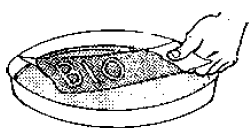
\includegraphics[width=0.4\textwidth]{./img/source/saliva-ink.png}
\end{center}

\begin{description*}
\item[Topic:]{Nutrition - Form II}
\item[Materials:]{Filter paper/toilet paper, starch solution, iodine solution, matches/cotton swabs}
\item[Setup:]{Prepare a starch solution by adding a teaspoon of maize/cassava flour to half a
cup of water. Bring to a boil, then allow to cool and filter the liquid through a cloth.}
\item[Procedure:]{Soak toilet paper in starch solution. Ask students to use saliva on a matchstick or cotton swab to write their names on the treated paper. Dip the paper in a very dilute iodine solution.}
%\item[Hazards:]{}
%\item[Questions:]{}
%\item[Observations:]{}
\item[Theory:]{The enzymes in the saliva digest the starch where it touches the paper.}
%\item[Applications:]{Enzyme action}
%\item[Notes:]{}
\end{description*}

\subsection{Swallowing Upside Down} % Shika 220, Source 64

\begin{center}
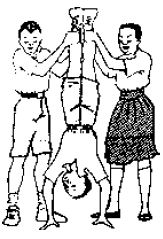
\includegraphics[width=0.35\textwidth]{./img/source/peristalsis.png}
\end{center}

\begin{description*}
\item[Topic:]{Peristalsis (Nutrition) - Form II}
\item[Materials:]{Drinking water/bread}
%\item[Setup:]{}
\item[Procedure:]{Drink a mouth full of water from a cup and swallow it. Then fill your mouth again, (without
swallowing) and with the help of two friends do a handstand. Then swallow while upside down. Also try with a small piece of bread}
%\item[Hazards:]{}
%\item[Questions:]{}
\item[Observations:]{You are able to swallow while upside down, but not as easily.}
\item[Theory:]{The peristalsis of the
esophagus works against the forces of gravity.}
%\item[Applications:]{}
%\item[Notes:]{}
\end{description*}

\subsection{Photosynthesis Model} % VSO 38

\begin{center}
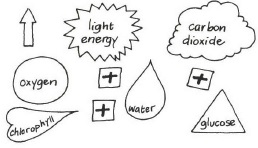
\includegraphics[width=0.45\textwidth]{./img/vso/photo-model.jpg}
\end{center}

\begin{description*}
\item[Topic:]{Photosynthesis (Nutrition) - Form II}
\item[Materials:]{Card/paper, matches}
%\item[Setup:]{}
\item[Procedure:]{Draw and cut out the symbols shown above. Then arrange them in the correct order to
show the chemical equation for photosynthesis. Use matchsticks for arrows and + symbols.}
%\item[Hazards:]{}
%\item[Questions:]{}
%\item[Observations:]{}
%\item[Theory:]{}
%\item[Applications:]{}
\item[Notes:]{Repeat the above procedure but replace the words in the shapes with the chemical
formulae of the substances involved. These may be written on the reverse side of the first set
of cards.}
\end{description*}

\subsection{Photosynthesis Equation Game} % VSO 39

\begin{center}
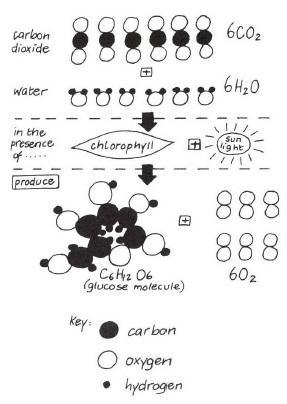
\includegraphics[width=0.45\textwidth]{./img/vso/photo-game.jpg}
\end{center}

\begin{description*}
\item[Topic:]{Photosynthesis (Nutrition) - Form II}
\item[Materials:]{Beans, stones, coins, bottle caps, etc.}
%\item[Setup:]{}
\item[Procedure:]{Arrange the items so they
represent the stages of
photosynthesis as shown in the
diagram.}
%\item[Hazards:]{}
%\item[Questions:]{}
%\item[Observations:]{}
%\item[Theory:]{}
%\item[Applications:]{}
%\item[Notes:]{}
\end{description*}

\subsection{Food Webs} % VSO 56

\begin{center}
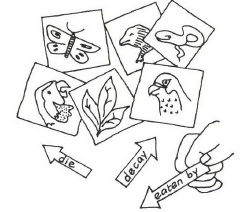
\includegraphics[width=0.4\textwidth]{./img/vso/food-webs.jpg}
\end{center}

\begin{description*}
\item[Topic:]{Balance of Nature - Form II}
\item[Materials:]{Card, pictures of animals and plants (optional)}
%\item[Setup:]{}
\item[Procedure:]{Either draw pictures of animals
and plants on cards or stick on
pictures cut out from magazines
etc. Make arrows and write on
them the links shown. Arrange
the cards and arrows to make a
food web.}
%\item[Hazards:]{}
%\item[Questions:]{}
%\item[Observations:]{}
%\item[Theory:]{}
%\item[Applications:]{}
%\item[Notes:]{}
\end{description*}

%\subsection{Osmosis/Active Transport Model} % Source 79
%
%\begin{center}
%\includegraphics[width=0.4\textwidth]{./img/vso/active-transport.jpg}
%\end{center}
%
%\begin{description*}
%\item[Topic:]{Transport - Form II}
%\item[Materials:]{Cardboard tray, matchboxes, peas/beans, bottle caps, tape}
%\item[Setup:]{Tape the bottoms of matchboxes to a tray as shown. The gaps between the boxes should allow small objects to pass (i.e. peas) but prevent
%movement of larger ones (soda bottle caps).}
%\item[Procedure:]{Place ten soda bottle caps and ten peas in one
%side of the tray and twenty peas in the other side. Shake the tray gently ten times. Count the
%peas in each side.}
%%\item[Hazards:]{}
%%\item[Questions:]{}
%%\item[Observations:]{}
%\item[Theory:]{The
%matchboxes and spaces between
%them represent a selectively
%permeable membrane. The spaces
%allow small objects through, but
%not larger ones. The peas
%represent water molecules which
%move freely. The bottle caps
%represent the larger glucose
%molecules which need to be
%placed in the matchbox drawers
%and actively pushed through to
%the other side.}
%%\item[Applications:]{}
%%\item[Notes:]{}
%\end{description*}

\subsection{Data on Pulse Rate}

\begin{center}
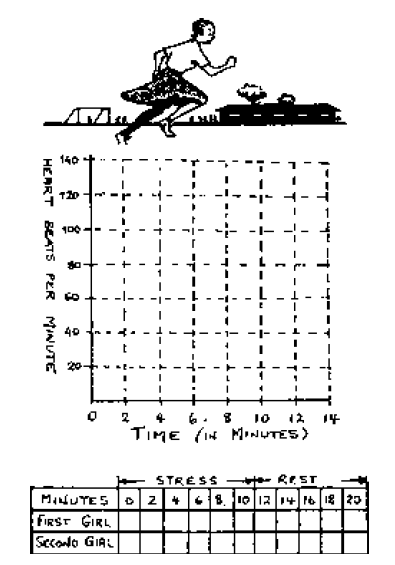
\includegraphics[width=0.4\textwidth]{./img/source/data-pulse.png}
\end{center}

\begin{description*}
\item[Topic:]{Transport - Form II}
%\item[Materials:]{}
%\item[Setup:]{}
\item[Procedure:]{Take the resting pulse rate of ten students, then ask them to run around the school
compound for two minutes. Take the pulse of each student at two minute intervals until the
pulse returns to normal. For each student plot a graph of pulse rate against time.}
%\item[Hazards:]{}
\item[Questions:]{Which pulse rate was the highest and which pulse returned to normal most quickly?}
\item[Observations:]{Each curve of pulse rate will be slightly different.}
\item[Theory:]{This is due to differences in levels of physical fitness of each student. The less fit ones
generally reach a higher pulse rate, which takes longer to return to normal.}
%\item[Applications:]{}
%\item[Notes:]{}
\end{description*}

\subsection{Breathing Model} % VSO 34

\begin{center}
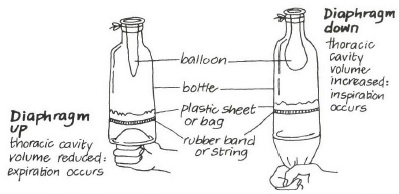
\includegraphics[width=0.49\textwidth]{./img/vso/breathing-model.jpg}
\end{center}

\begin{description*}
\item[Topic:]{Gas Exchange - Form II}
\item[Materials:]{Plastic bottle, balloons, plastic bag, string/rubber band, straw}
%\item[Setup:]{}
\item[Procedure:]{Cut the bottom off a plastic
bottle. Attach a balloon over the
bottle mouth so it hangs inside.
Fix a piece of plastic bag over the
cut base end using string or a rubber band. (Optional: Fix a straw through the bottle top and attach 1 or 2 balloons to the end inside the bottle.)}
%\item[Hazards:]{}
%\item[Questions:]{}
\item[Observations:]{Pulling the plastic bag down causes the balloon to inflate; pushing it up causes the balloon the deflate.}
\item[Theory:]{The balloon(s) represents the lung(s), the plastic bag the diaphragm, the bottle the thoracic cavity (and the straw the esophagus). Pulling the plastic sheet down causes an expansion of the cavity bringing about inspiration and causing the balloon to inflate. Pushing the sheet up reduces the volume of the cavity, causing expiration and the balloon to deflate.}
%\item[Applications:]{}
\item[Notes:]{Tell students that this model does not show the expansion and contraction of the rib cage with breathing.}
\end{description*}

\subsection{Neuron Models}

\begin{center}
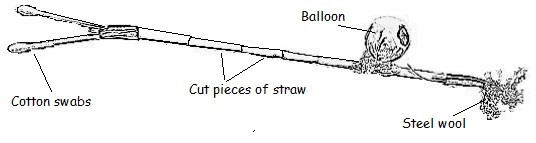
\includegraphics[width=0.49\textwidth]{./img/neuron-model.jpg}
\end{center}

\begin{description*}
\item[Topic:]{Coordination - Form III}
\item[Materials:]{Straight stick/bamboo skewer, straws, tape, balloon, steel wool, cotton swabs, scissors}
%\item[Setup:]{}
\item[Procedure:]{Cut several short lengths of straw and place them over a bamboo skewer or straight stick. Fill a balloon slightly and tape it a few centimetres from one end. Draw a large black dot on the balloon. Attach steel wool and cotton swabs to the ends as shown.}
%\item[Hazards:]{}
%\item[Questions:]{}
%\item[Observations:]{}
%\item[Theory:]{}
%\item[Applications:]{}
\item[Notes:]{Use similar materials to make models of other types of neurons.}
\end{description*}

\subsection{Taste Map}

\begin{center}
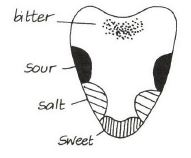
\includegraphics[width=0.35\textwidth]{./img/vso/taste-map.jpg}
\end{center}

\begin{description*}
\item[Topic:]{Coordination - Form III}
\item[Materials:]{4 glasses, spoon, coffee, vinegar, salt, sugar, water}
\item[Setup:]{Prepare the 4 taste solutions as follows:
\begin{itemize}
\item Bitter: Lemon peel, coffee dissolved in water or strong cold tea
\item Sour:Vinegar or lime juice
\item Salty: Salt dissolved in water
\item Sweet: Sugar dissolved in water
\end{itemize}}
%\item[Bitter:]{Lemon peel, coffee dissolved in water or strong cold tea}
%\item[Sour:]{Vinegar or lime juice}
%\item[Salty:]{Salt dissolved in water}
%\item[Sweet:]{Sugar dissolved in water}
\item[Procedure:]{Use a spoon to pour a small amount of each solution in students' hands, one at a time. Have them taste the solution and describe the taste, as well as where on their tongues the taste in found.}
%\item[Questions:]{}
%\item[Observations:]{}
\item[Theory:]{The tongue has receptors for different tastes in different places. Make a diagram of the tongue as shown to display in the class.}
%\item[Applications:]{}
%\item[Notes:]{}
\end{description*}

\subsection{DNA Model Game} % VSO 52

\begin{center}
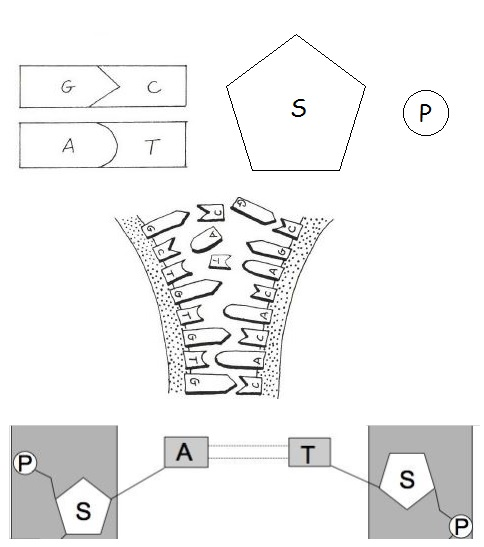
\includegraphics[width=0.4\textwidth]{./img/dna-game.jpg}
\end{center}

\begin{description*}
\item[Topic:]{Genetics - Form IV}
\item[Materials:]{Card/paper, scissors}
\item[Setup:]{Cut out pieces of card to
represent the paired bases, sugars and phosphate groups.}
\item[Procedure:]{Construct a DNA model by correctly joining the parts of the nucleotide. The phosphate group (P) should be atop the deoxyribose sugar (S) and the
base pairs should bond to the deoxyribose sugar as shown. Students must match the bases to
`zip up' the DNA molecule.}
%\item[Hazards:]{}
%\item[Questions:]{}
\item[Observations:]{The bases
always combine in the same pairs:
thymine with adenine and
cytosine with guanine.}
\item[Theory:]{DNA is a double-stranded helical (spiral) molecular chain that is found in the nucleus of the cell. It contains the genetic information of organisms. DNA is made up of many \emph{nucleotides}. The components of a DNA nucleotide are a deoxyribose sugar, phosphoric acid, and an organic base. The four bases of DNA are guanine, cytosine, adenine, and thymine. In humans, DNA determines physical features such as the colour of the skin, eyes, and hair as well as a person's height and the presence or absence of genetic disorders.}
%\item[Applications:]{}
%\item[Notes:]{}
\end{description*}

\subsection{Natural Selection Game} % NEW - PIC!!!

%\begin{center}
%\includegraphics[width=0.4\textwidth]{./img/.png}
%\end{center}

\begin{description*}
\item[Topic:]{Evolution - Form IV}
\item[Materials:]{Rice, beans, 3 bottles, 6 clothespins, 6 plastic forks, 6 plastic spoons}
%\item[Setup:]{}
\item[Procedure:]{Get 6 students. Give 2 of them forks, 2 of them spoons, and 2 of them clothespins. Give each pair a beaker or cut off bottle. Spread the beans and rice in the middle of the table. Each team has 20 seconds to collect beans and rice and place them into the beakers. The two teams with the most beans and rice in their beakers will advance to the next round. Continue with round 2 for 20 seconds. The team with the most beans and rice in their beaker wins.}
%\item[Hazards:]{}
%\item[Questions:]{}
\item[Observations:]{Students using spoons should be able to gather the most beans and rice.}
\item[Theory:]{There is always competition or struggle between organisms for limited resources such as food, space, etc. Only well adapted organisms survive while the less adapted are eliminated (survival of the fittest).}
%\item[Applications:]{}
%\item[Notes:]{}
\end{description*}


%\pagebreak
%
%\subsection{Robotic Hand}
%
%\begin{center}
%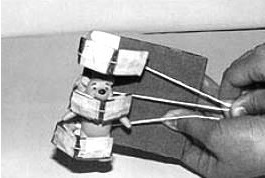
\includegraphics[width=0.4\textwidth]{./img/robotic-hand-use.jpg}
%\end{center}
%
%\begin{description*}
%\item[Topic:]{Movement - Form III}
%\item[Materials:]{Rubber bands, straws, cardboard, string, masking tape, scissors}
%%\item[Setup:]{}
%%\item[Procedure:]{}
%%\item[Hazards:]{}
%%\item[Questions:]{}
%%\item[Observations:]{}
%%\item[Theory:]{}
%%\item[Applications:]{}
%%\item[Notes:]{}
%\end{description*}
%
%\subsubsection{Hand Structure}
%
%\begin{center}
%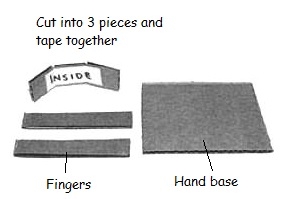
\includegraphics[width=0.4\textwidth]{./img/robotic-hand-1.jpg}
%\end{center}
%
%\begin{description*}
%%\item[Subtopic:]{}
%%\item[Materials:]{}
%%\item[Setup:]{}
%\item[Procedure:]{Cut a piece of cardboard about 10~cm $\times$ 10~cm. This is the ``palm'' of the hand. Cut three pieces of cardboard about 2 cm $\times$ 9 cm. These are the ``fingers''. Cut one finger into three equal pieces. Place the three finger pieces back together and put a piece of tape over the two
%finger joints. Label the tape ``inside''.}
%%\item[Hazards:]{}
%%\item[Questions:]{}
%%\item[Observations:]{}
%%\item[Theory:]{}
%%\item[Applications:]{}
%%\item[Notes:]{}
%\end{description*}
%
%\subsubsection{Fingers}
%
%\begin{center}
%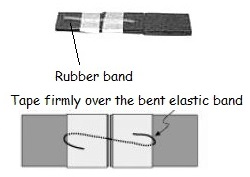
\includegraphics[width=0.35\textwidth]{./img/robotic-hand-finger.jpg}
%\end{center}
%
%\begin{description*}
%%\item[Subtopic:]{}
%%\item[Materials:]{}
%%\item[Setup:]{}
%\item[Procedure:]{Cut a piece of elastic about 5 cm long. Turn the finger over (inside facing down) and place the elastic across the middle of the first joint. Tape the elastic on either side of the joint, leaving the ends of the elastic untaped (rip tape to make it thin). Bend the ends of the elastic as shown and tape firmly. This will help prevent the elastic from slipping. Repeat for the second joint.}
%%\item[Hazards:]{}
%%\item[Questions:]{}
%%\item[Observations:]{}
%%\item[Theory:]{}
%%\item[Applications:]{}
%%\item[Notes:]{}
%\end{description*}
%
%\subsubsection{Attach Fingers}
%
%\begin{center}
%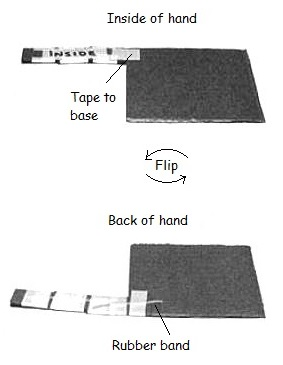
\includegraphics[width=0.45\textwidth]{./img/robotic-hand-3.jpg}
%\end{center}
%
%\begin{description*}
%%\item[Subtopic:]{}
%%\item[Materials:]{}
%%\item[Setup:]{}
%\item[Procedure:]{Tape the finger (inside up) onto the palm. Turn the hand over and fasten the last finger joint to the palm using the same method as above.}
%%\item[Hazards:]{}
%%\item[Questions:]{}
%%\item[Observations:]{}
%%\item[Theory:]{}
%%\item[Applications:]{}
%%\item[Notes:]{}
%\end{description*}
%
%\subsubsection{Moving Joints}
%
%\begin{center}
%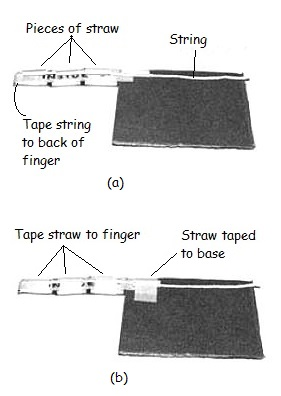
\includegraphics[width=0.45\textwidth]{./img/robotic-hand-4.jpg}
%\end{center}
%
%\begin{description*}
%%\item[Subtopic:]{}
%%\item[Materials:]{}
%%\item[Setup:]{}
%\item[Procedure:]{Cut a piece of string about 35 cm long and tape one end firmly over the end of
%the finger. Cut four pieces of straw each about 2 cm long and thread them onto the string. Tape three of the straws in the middle of each of the finger sections. Tape the last straw to the palm as shown. }
%%\item[Hazards:]{}
%%\item[Questions:]{}
%%\item[Observations:]{}
%%\item[Theory:]{}
%%\item[Applications:]{}
%%\item[Notes:]{}
%\end{description*}
%
%\subsubsection{Completing the Hand}
%
%\begin{center}
%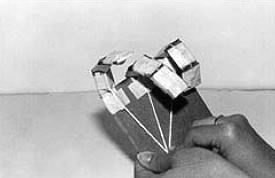
\includegraphics[width=0.4\textwidth]{./img/robotic-hand-final.jpg}
%\end{center}
%
%\begin{description*}
%%\item[Subtopic:]{}
%%\item[Materials:]{}
%%\item[Setup:]{}
%\item[Procedure:]{Repeat the steps above for the last two fingers. When finished, operate the hand by pulling the strings. You should be able to pick up empty soda cans and other light objects with your hand.}
%%\item[Hazards:]{}
%%\item[Questions:]{}
%%\item[Observations:]{}
%%\item[Theory:]{}
%%\item[Applications:]{}
%%\item[Notes:]{}
%\end{description*}


\end{multicols}